% Asset ID: FA22MomentumImpulseFoundationsForRestitutionTikZ-001
% Asset type: TikZ diagram
% Topic ID: FA22MomentumImpulseFoundationsForRestitution
% Lesson file: FA22_momentum_impulse_foundations_for_restitution_lesson.md
% Related lesson section: Section 9: Visual Asset Integration
% Source: transcript sign convention warnings and worked examples
% Purpose: Show that either direction may be chosen positive, provided signs are used consistently.

\documentclass[tikz,border=8pt]{standalone}
\usepackage{amsmath}
\usepackage{xcolor}
\usetikzlibrary{arrows.meta, positioning, calc}
\definecolor{Canvas}{HTML}{FAF9F6}
\definecolor{Panel}{HTML}{FFFFF0}
\definecolor{Line}{HTML}{E5E5EA}
\definecolor{Accent}{HTML}{C5A059}
\definecolor{SoftPink}{HTML}{FBEFEF}
\definecolor{Text}{HTML}{2C2C2E}
\definecolor{Muted}{HTML}{6B6B70}
\begin{document}
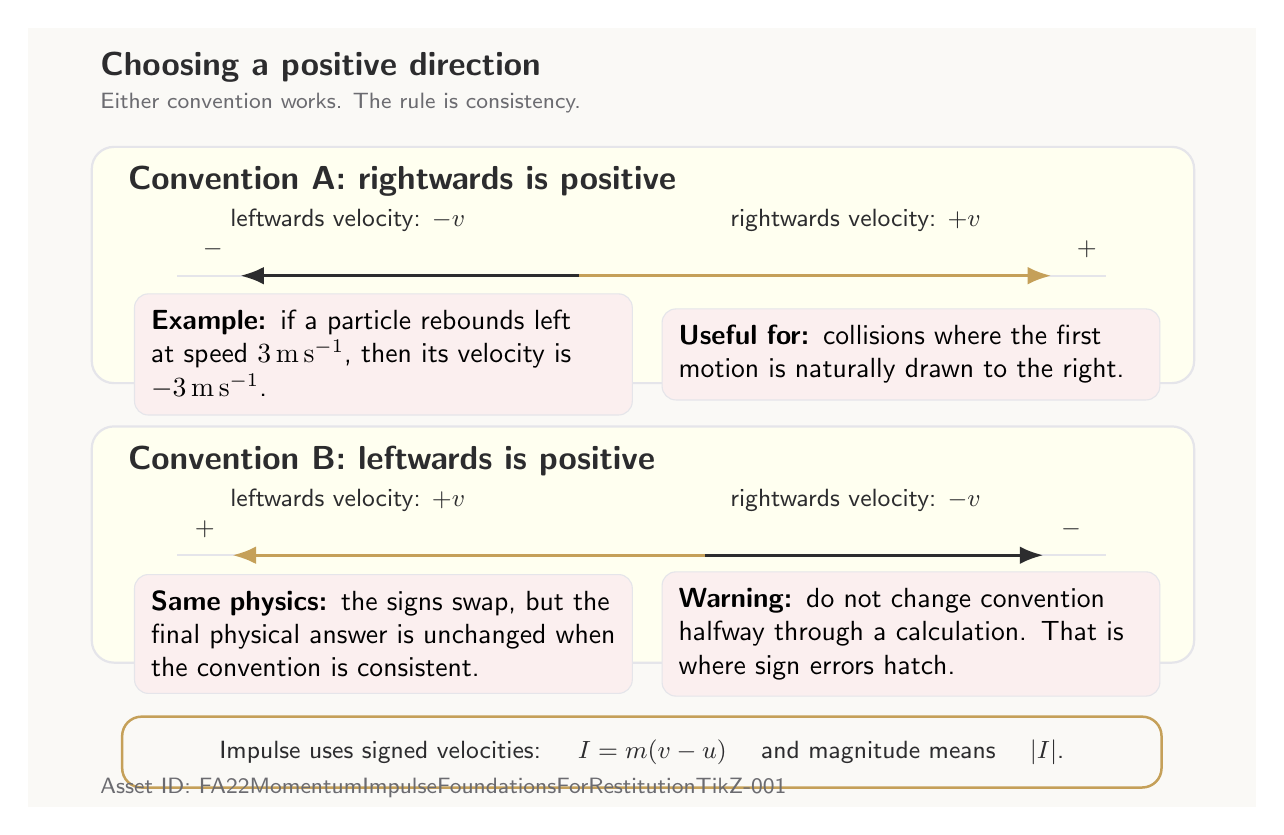
\begin{tikzpicture}[font=\sffamily,>=Latex,velocity/.style={-{Latex[length=3mm]}, very thick, draw=Text},accentarrow/.style={-{Latex[length=3mm]}, very thick, draw=Accent},faintline/.style={draw=Line, line width=0.8pt},panel/.style={draw=Line, fill=Panel, rounded corners=8pt, line width=0.8pt},note/.style={draw=Line, fill=SoftPink, rounded corners=5pt, inner sep=6pt},labeltext/.style={text=Text, font=\sffamily\small},titletext/.style={text=Text, font=\sffamily\bfseries\large},smallmuted/.style={text=Muted, font=\sffamily\footnotesize}]
\fill[Canvas] (-0.8,-5.4) rectangle (14.8,4.5);
\node[titletext, anchor=west] at (0,4.0) {Choosing a positive direction};
\node[smallmuted, anchor=west] at (0,3.55) {Either convention works. The rule is consistency.};
\node[panel, minimum width=14cm, minimum height=3cm, anchor=north west] at (0,3.0) {};
\node[titletext, anchor=west] at (0.35,2.55) {Convention A: rightwards is positive};
\draw[faintline] (1.1,1.35) -- (12.9,1.35);
\draw[accentarrow] (6.2,1.35) -- (12.2,1.35);
\draw[velocity] (6.2,1.35) -- (1.9,1.35);
\node[labeltext] at (12.65,1.68) {$+$}; \node[labeltext] at (1.55,1.68) {$-$};
\node[labeltext, anchor=west] at (8.0,2.05) {rightwards velocity: $+v$};
\node[labeltext, anchor=west] at (1.65,2.05) {leftwards velocity: $-v$};
\node[note, anchor=west, text width=5.9cm] at (0.55,0.35) {\textbf{Example:} if a particle rebounds left at speed $3\,\mathrm{m\,s^{-1}}$, then its velocity is $-3\,\mathrm{m\,s^{-1}}$.};
\node[note, anchor=west, text width=5.9cm] at (7.25,0.35) {\textbf{Useful for:} collisions where the first motion is naturally drawn to the right.};
\node[panel, minimum width=14cm, minimum height=3cm, anchor=north west] at (0,-0.55) {};
\node[titletext, anchor=west] at (0.35,-1.0) {Convention B: leftwards is positive};
\draw[faintline] (1.1,-2.2) -- (12.9,-2.2);
\draw[accentarrow] (7.8,-2.2) -- (1.8,-2.2);
\draw[velocity] (7.8,-2.2) -- (12.1,-2.2);
\node[labeltext] at (1.45,-1.87) {$+$}; \node[labeltext] at (12.45,-1.87) {$-$};
\node[labeltext, anchor=west] at (1.65,-1.5) {leftwards velocity: $+v$};
\node[labeltext, anchor=west] at (8.0,-1.5) {rightwards velocity: $-v$};
\node[note, anchor=west, text width=5.9cm] at (0.55,-3.2) {\textbf{Same physics:} the signs swap, but the final physical answer is unchanged when the convention is consistent.};
\node[note, anchor=west, text width=5.9cm] at (7.25,-3.2) {\textbf{Warning:} do not change convention halfway through a calculation. That is where sign errors hatch.};
\node[draw=Accent, fill=Canvas, rounded corners=7pt, line width=0.9pt, minimum width=13.2cm, minimum height=0.9cm] at (7,-4.7) {};
\node[labeltext] at (7,-4.7) {Impulse uses signed velocities: \quad $I=m(v-u)$ \quad and magnitude means \quad $|I|$.};
\node[smallmuted, anchor=west] at (0,-5.15) {Asset ID: FA22MomentumImpulseFoundationsForRestitutionTikZ-001};
\end{tikzpicture}
\end{document}
